\documentclass[10pt,a4paper,twocolumn]{article}

% bibliotecas
\usepackage[utf8]{inputenc}
\usepackage[brazil]{babel}
\usepackage{graphicx}
\usepackage{amsmath,amsfonts,amsthm}

% comandos
\newcommand{\chaves}[1] {{\left \{ {#1} \right \}}}
\newcommand{\parenteses}[1] {\left ( {#1} \right )}
\newcommand{\barras}[1] {{\left \| {#1} \right \|}}
\newcommand{\Prob}[1] {\mathbb{P}\chaves{#1}}

% documento
\title{Relatório da implementação e testes do k-NN}
\author{\small{Cássio Jandir Pagnoncelli\footnote{cjp07@inf.ufpr.br}}}

\begin{document}
\flushbottom
\maketitle

%--- texto
\section{Introdução}

  O algoritmo k-NN é um classificador paramétrico que se baseia nos vizinhos
  mais próximos do novo elemento a ser classificado. Em princípio, esse
  classificador tem $k$ (ímpar positivo) como único parâmetro. A classe desse
  novo elemento é determinada pela classe mais frequente dentre as classes dos
  $k$ elementos mais próximos, segundo a função que determina a distância, desse
  novo elemento até seus vizinhos.

  \subsection{Empate em frequência de classes}

    Eventualmente pode não existir apenas uma classe mais frequente, mas um
    conjunto delas. Como, nesse caso, é necessário tomar uma decisão de qual
    classe atribuir a esse novo elemento, essa classe será a de menor índice
    dentre as que empataram em frequência.

  \subsection{Cálculo de distância}

    Existem diversas formas de determinar a distância entre dois pontos
    $x~=~(x_1,x_2,x_3,\ldots,x_n)$ e $y~=~(y_1,y_2,y_3,\ldots,y_n)$. A mais
    usual é a distância euclidiana, que é a menor distância entre dois pontos
    num espaço vetorial euclidiano, dado por

    \begin{equation*}
      d(x, y) = \sqrt{\sum_{i=1}^n \parenteses{x_i - y_i}^2}
    \end{equation*}

    Entretanto, foram implementados outros métodos para determinar a distância
    entre dois pontos quaisquer, descritos a seguir.

    \subsubsection*{Distância Manhattan}

    É adequado quando a distância entre $x$ e $y$ por meio da distância
    euclidiana é infactível, que é justamente a distância da hipotenusa no
    triângulo formado pelos pontos $x$, $y$ e o ponto
    $(\min(x_1, y_1), \min(x_2, y_2), \min(x_3, y_3), \ldots, \min(x_n, y_n))$.
    A distância Manhattan é justamente a medida da soma dos catetos desse
    triângulo, calculada assim

    \begin{equation*}
      d(x, y) = \sum_{i=1}^n \barras{x_i - y_i}.
    \end{equation*}

    \subsubsection*{Distância Chebyschev}

    É análogo ao cálculo da distância Manhattan, mas ao invés de levar em
    conta a distância de todos os catetos, leva em conta ---e é determinado---
    unicamente pela distância do maior cateto; ou seja,

    \begin{equation*}
      d(x, y) = \max \chaves{x_i - y_i \colon 1 \leq i \leq n}.
    \end{equation*}

    \subsubsection*{Distância Minkowski}

    Trata-se uma generalização dos cálculos de distâncias euclidiana, Manhattan
    e Chebyschev e é dado por

    \begin{equation*}
      d(x, y) = \parenteses{\sum_{i=1}^n \barras{x_i - y_i}^p}^{\frac{1}{p}}.
    \end{equation*}
    
    Quando $p=1$ e $p=2$, claramente $d(x, y)$ é equivalente às funções de
    cálculo de distâncias Manhattan e euclidiana, respectivamente. Por outro
    lado, ao passo que $p$ se aproxima do tamanho da amostra, $d(x, y)$
    apresenta um erro cada vez menor em relação à distância Chebyschev; isto é,
    no limite, quando $p$ se iguala ao tamanho da amostra, $d(x, y)$ é
    equivalente a distância Chebyschev.

    \subsection{Normalização dos dados}

    Em se tratando dos dados, cada eixo (ou característica) do conjunto de dados
    é valorado sobre uma escala. Essa escala pode ser diferente dos demais
    eixos, gerando distorções na real distância entre dois pontos quaisquer. Por
    isso, é fornecido a opção de normalizar os dados numa escala linear 
    $[0..1]$. (Para uso dessa opção, veja o arquivo {\sf LEIAME} que acompanha
    o código-fonte do k-NN.)

  \section{Resultado dos experimentos}

  As taxas de acerto, que determinam a relação entre classificações corretas e
  totais feitas pelo k-NN, apresenta uma certa homogeneidade para valores
  pequenos de $k$. A primeira tabela, dentre as duas seguintes, mostra as
  melhores taxas de acerto ---para cada uma das abordagens no cálculo de
  distância entre dois pontos quaisquer---, enquanto a segunda tabela mostra os
  respectivos valores de $k$ associados em que a taxa de acerto é máxima
  ---novamente, para cada uma das abordagens de cálculo de distância entre dois
  pontos quaisquer.

  \begin{table}[ht]
    \caption{{\scriptsize Melhores taxas de acerto}}
    \centering
    \begin{tabular}{c c c}
      \hline\hline 
      % cabeçalho
      {\scriptsize Função distância} 
      & {\scriptsize não-normalizado} 
      & {\scriptsize normalizado} \\ [0.5ex]
      % corpo
      \hline
      {\scriptsize Euclidiana}     & \small 0.908 & \small 0.907 \\
      {\scriptsize Manhattan}      & \small 0.950 & \small 0.947 \\
      {\scriptsize Chebyschev}     & \small 0.879 & \small 0.880 \\
      {\scriptsize Minkowski(p=3)} & \small 0.879 & \small 0.880 \\
      {\scriptsize Minkowski(p=5)} & \small 0.879 & \small 0.881 \\
      {\scriptsize Minkowski(p=6)} & \small 0.880 & \small 0.882 \\
      [1ex]
      \hline
    \end{tabular}
  \end{table}

  \begin{table}[ht]
    \caption{{\scriptsize Valores ótimos de $k$}}
    \centering
    \begin{tabular}{c c c}
      \hline\hline 
      % cabeçalho
      {\scriptsize Função distância} 
      & {\scriptsize não-normalizado} 
      & {\scriptsize normalizado} \\ [0.5ex]
      % corpo
      \hline
      {\scriptsize Euclidiana}     & \small 27 & \small 51 \\
      {\scriptsize Manhattan}      & \small 21 & \small 57 \\
      {\scriptsize Chebyschev}     & \small  1 & \small  1 \\
      {\scriptsize Minkowski(p=3)} & \small  1 & \small  1 \\
      {\scriptsize Minkowski(p=5)} & \small  1 & \small  1 \\
      {\scriptsize Minkowski(p=6)} & \small  1 & \small  1 \\
      [1ex]
      \hline
    \end{tabular}
  \end{table}
  

    \subsection{Taxas de acerto}

      Estas são as taxas de acerto para diferentes valores de $k$ em que os
      dados não estão normalizados

      \includegraphics[scale=0.33]{graficos/euclidiana_0.ps}
      \includegraphics[scale=0.33]{graficos/manhattan_0.ps}
      \includegraphics[scale=0.33]{graficos/chebyschev_0.ps}
      \includegraphics[scale=0.33]{graficos/minkowski_3_0.ps}
      \includegraphics[scale=0.33]{graficos/minkowski_5_0.ps}
      \includegraphics[scale=0.33]{graficos/minkowski_6_0.ps}

      e estas são as mesmas taxas para os mesmos dados, porém normalizados
      
      \includegraphics[scale=0.33]{graficos/euclidiana_1.ps}
      \includegraphics[scale=0.33]{graficos/manhattan_1.ps}
      \includegraphics[scale=0.33]{graficos/chebyschev_1.ps}
      \includegraphics[scale=0.33]{graficos/minkowski_3_1.ps}
      \includegraphics[scale=0.33]{graficos/minkowski_5_1.ps}
      \includegraphics[scale=0.33]{graficos/minkowski_6_1.ps}

    \subsection{Matrizes de confusão}

      As matrizes de confusão explicitam a adequação do classificador sobre as
      classe; isto é, medem a qualidade do classificador para cada uma das
      classes, no escopo da base de treinamento. As seguintes matrizes de
      confusão são justamente as matrizes associadas aos gráficos anteriores;
      ou seja, são as matrizes para os quais o valor de $k$ é ótimo.
      (O label da matriz indica a função usada no cálculo de distância; 
      o índice indica se os dados são (norm) ou não normalizados (não-norm);
      um elemento contado na posição $M[lin][col]$ representa que o k-NN
      classificou tal elemento como sendo da classe $lin$ enquanto seu registro
      aponta como sendo da classe $col$; e, as $n$ classes são dispostas de
      forma crescente para baixo e para a direita na matriz.)

      Usando a função euclidiana, com dados não-normalizados, temos
      
      \begin{equation*}
        \textsf{euclidiana}_\text{não-norm}~=~ \left [
        \begin{smallmatrix}
          96 &  1 &  0 &  1 &  0 &  0 &  0 &  0 &  8 &  0 \\
           0 & 86 &  0 &  0 &  0 &  0 &  0 &  0 &  1 &  0 \\ 
           0 &  3 & 88 &  8 &  0 &  0 &  1 &  0 &  1 &  0 \\ 
           3 &  0 &  5 & 84 &  0 &  2 &  0 &  0 &  4 &  0 \\ 
           0 &  1 &  0 &  1 & 97 &  1 &  0 &  0 &  2 &  1 \\ 
           0 &  1 &  1 &  0 &  0 & 93 &  1 &  0 &  3 &  0 \\ 
           0 &  1 &  2 &  3 &  1 &  1 & 98 &  0 &  0 &  0 \\ 
           0 &  1 &  0 &  0 &  0 &  0 &  0 & 96 &  0 &  4 \\ 
           0 &  5 &  4 &  2 &  1 &  0 &  0 &  0 & 76 &  1 \\ 
           1 &  1 &  0 &  1 &  1 &  3 &  0 &  4 &  5 & 94 \\ 
        \end{smallmatrix} \right ]
      \end{equation*}
      enquanto com dados normalizados temos
      \begin{equation*}
        \textsf{euclidiana}_\text{norm}~=~ \left [
        \begin{smallmatrix}
          90 &  3 &  0 &  0 &  0 &  0 &  0 &  0 &  0 &  0 \\
           0 & 88 &  0 &  0 &  0 &  0 &  0 &  0 &  1 &  0 \\ 
           0 &  3 & 87 &  8 &  0 &  0 &  1 &  0 &  1 &  0 \\ 
           1 &  0 &  6 & 85 &  0 &  3 &  0 &  0 &  3 &  0 \\ 
           1 &  0 &  0 &  1 & 96 &  0 &  0 &  1 &  3 &  1 \\ 
           0 &  1 &  1 &  0 &  0 & 93 &  1 &  0 &  4 &  0 \\ 
           3 &  1 &  3 &  2 &  1 &  1 & 97 &  1 &  0 &  0 \\ 
           0 &  1 &  0 &  0 &  0 &  0 &  0 & 96 &  0 &  4 \\ 
           4 &  2 &  3 &  2 &  1 &  0 &  0 &  0 & 82 &  2 \\ 
           1 &  1 &  0 &  2 &  2 &  3 &  1 &  2 &  6 & 93 \\ 
        \end{smallmatrix} \right ]
      \end{equation*}
      
      Para a função Manhattan, com dados não-normalizados, temos
      \begin{equation*}
        \textsf{Manhattan}_\text{não-norm}~=~ \left [
        \begin{smallmatrix}
          98 &  0 &  0 &  1 &  0 &  0 &  0 &  0 &  7 &  0 \\
           0 & 92 &  0 &  0 &  0 &  0 &  0 &  0 &  1 &  0 \\ 
           0 &  3 & 94 &  3 &  0 &  0 &  0 &  0 &  0 &  0 \\ 
           1 &  0 &  1 & 94 &  0 &  2 &  0 &  0 &  1 &  0 \\ 
           0 &  0 &  0 &  0 & 99 &  0 &  0 &  1 &  1 &  0 \\ 
           0 &  1 &  0 &  0 &  0 & 97 &  1 &  0 &  0 &  0 \\ 
           0 &  0 &  1 &  1 &  1 &  0 & 99 &  0 &  2 &  0 \\ 
           0 &  0 &  0 &  0 &  0 &  0 &  0 & 98 &  0 &  3 \\ 
           0 &  3 &  4 &  0 &  0 &  0 &  0 &  0 & 82 &  0 \\ 
           1 &  1 &  0 &  1 &  0 &  1 &  0 &  1 &  6 & 97 \\ 
        \end{smallmatrix} \right ]
      \end{equation*}
      enquanto com os dados normalizados temos
      \begin{equation*}
        \textsf{Manhattan}_\text{norm}~=~ \left [
        \begin{smallmatrix}
          87 &  3 &  0 &  0 &  0 &  0 &  0 &  0 &  0 &  0 \\
           2 & 91 &  0 &  0 &  0 &  0 &  0 &  0 &  0 &  0 \\ 
           0 &  3 & 94 &  2 &  0 &  0 &  0 &  0 &  0 &  0 \\ 
           1 &  0 &  1 & 95 &  0 &  1 &  0 &  0 &  2 &  0 \\ 
           0 &  0 &  0 &  0 & 99 &  0 &  0 &  0 &  1 &  1 \\ 
           0 &  1 &  1 &  0 &  0 & 99 &  1 &  0 &  0 &  0 \\ 
           3 &  0 &  1 &  1 &  1 &  0 & 99 &  0 &  0 &  0 \\ 
           0 &  0 &  0 &  0 &  0 &  0 &  0 & 98 &  0 &  6 \\ 
           7 &  1 &  3 &  1 &  0 &  0 &  0 &  0 & 92 &  0 \\ 
           0 &  1 &  0 &  1 &  0 &  0 &  0 &  2 &  5 & 93 \\ 
        \end{smallmatrix} \right ]
      \end{equation*}

      Para a função Chebyschev, com dados não-normalizados, temos
      \begin{equation*}
        \textsf{Chebyschev}_\text{não-norm}~=~ \left [
        \begin{smallmatrix}
          90 &  0 &  0 &  2 &  0 &  1 &  2 &  0 &  2 &  0 \\
           0 & 88 &  1 &  0 &  1 &  1 &  0 &  0 &  2 &  0 \\ 
           0 &  4 & 85 &  6 &  1 &  1 &  1 &  0 &  2 &  0 \\ 
           3 &  1 &  6 & 81 &  0 &  2 &  1 &  2 &  2 &  1 \\ 
           0 &  0 &  0 &  0 & 91 &  1 &  1 &  0 &  0 &  3 \\ 
           2 &  3 &  3 &  5 &  1 & 92 &  1 &  1 & 10 &  3 \\ 
           3 &  1 &  1 &  4 &  1 &  1 & 94 &  0 &  3 &  0 \\ 
           1 &  0 &  0 &  0 &  1 &  0 &  0 & 95 &  2 &  3 \\ 
           0 &  2 &  3 &  0 &  1 &  1 &  0 &  0 & 74 &  1 \\ 
           1 &  1 &  1 &  2 &  3 &  0 &  0 &  2 &  3 & 87 \\ 
        \end{smallmatrix} \right ]
      \end{equation*}
      enquanto com os dados normalizados temos
      \begin{equation*}
        \textsf{Chebyschev}_\text{norm}~=~ \left [
        \begin{smallmatrix}
          93 &  5 &  0 &  2 &  0 &  1 &  1 &  0 &  1 &  0 \\
           0 & 85 &  1 &  0 &  1 &  1 &  0 &  0 &  2 &  0 \\ 
           0 &  4 & 85 &  6 &  1 &  1 &  1 &  0 &  2 &  0 \\ 
           1 &  1 &  6 & 81 &  0 &  2 &  2 &  2 &  2 &  1 \\ 
           0 &  0 &  0 &  0 & 91 &  1 &  1 &  1 &  0 &  3 \\ 
           3 &  3 &  3 &  5 &  1 & 92 &  1 &  1 & 10 &  3 \\ 
           1 &  0 &  1 &  4 &  1 &  1 & 94 &  0 &  4 &  0 \\ 
           0 &  0 &  0 &  0 &  1 &  0 &  0 & 95 &  2 &  3 \\ 
           0 &  1 &  3 &  0 &  1 &  1 &  0 &  0 & 75 &  1 \\ 
           2 &  1 &  1 &  2 &  3 &  0 &  0 &  2 &  3 & 89 \\ 
        \end{smallmatrix} \right ]
      \end{equation*}

      Para a função Minkowski, com p=3 e dados não-normalizados, temos
      \begin{equation*}
        \textsf{Minkowski(p=3)}_\text{não-norm}~=~ \left [
        \begin{smallmatrix}
          93 &  0 &  2 &  3 &  0 &  1 &  2 &  0 &  3 &  0 \\
           0 & 88 &  1 &  0 &  1 &  1 &  0 &  0 &  2 &  1 \\ 
           0 &  3 & 84 &  6 &  0 &  1 &  1 &  0 &  2 &  0 \\ 
           3 &  1 &  7 & 83 &  0 &  2 &  1 &  2 &  3 &  0 \\ 
           0 &  1 &  0 &  0 & 93 &  0 &  0 &  1 &  2 &  3 \\ 
           2 &  3 &  3 &  5 &  1 & 95 &  1 &  0 &  5 &  3 \\ 
           1 &  1 &  0 &  1 &  1 &  0 & 95 &  0 &  2 &  0 \\ 
           0 &  0 &  0 &  0 &  0 &  0 &  0 & 95 &  2 &  5 \\ 
           0 &  3 &  3 &  0 &  1 &  0 &  0 &  0 & 76 &  0 \\ 
           1 &  0 &  0 &  2 &  3 &  0 &  0 &  2 &  3 & 88 \\ 
        \end{smallmatrix} \right ]
      \end{equation*}
      enquanto com os dados normalizados temos
      \begin{equation*}
        \textsf{Minkowski(p=3)}_\text{norm}~=~ \left [
        \begin{smallmatrix}
          93 &  4 &  0 &  2 &  0 &  1 &  1 &  0 &  0 &  0 \\
           0 & 87 &  1 &  0 &  1 &  1 &  0 &  0 &  2 &  1 \\ 
           0 &  3 & 84 &  6 &  0 &  1 &  2 &  0 &  2 &  0 \\ 
           2 &  1 &  8 & 83 &  0 &  2 &  1 &  2 &  5 &  0 \\ 
           0 &  1 &  0 &  0 & 93 &  0 &  0 &  1 &  2 &  3 \\ 
           2 &  3 &  4 &  5 &  1 & 95 &  1 &  0 &  6 &  3 \\ 
           1 &  0 &  0 &  2 &  1 &  0 & 95 &  0 &  2 &  0 \\ 
           1 &  0 &  0 &  0 &  0 &  0 &  0 & 95 &  2 &  5 \\ 
           1 &  1 &  3 &  0 &  1 &  0 &  0 &  0 & 76 &  0 \\ 
           0 &  0 &  0 &  2 &  3 &  0 &  0 &  2 &  3 & 88 \\ 
        \end{smallmatrix} \right ]
      \end{equation*}

      Para a função Minkowski, com p=5 e dados não-normalizados, temos
      \begin{equation*}
        \textsf{Minkowski(p=5)}_\text{não-norm}~=~ \left [
        \begin{smallmatrix}
          89 &  0 &  2 &  2 &  0 &  1 &  3 &  0 &  2 &  0 \\
           0 & 87 &  1 &  0 &  1 &  1 &  0 &  0 &  2 &  1 \\ 
           0 &  4 & 85 &  6 &  1 &  2 &  0 &  0 &  2 &  0 \\ 
           3 &  1 &  6 & 82 &  0 &  2 &  1 &  2 &  4 &  0 \\ 
           0 &  1 &  0 &  0 & 91 &  0 &  0 &  1 &  2 &  4 \\ 
           3 &  3 &  3 &  5 &  2 & 92 &  1 &  0 &  7 &  3 \\ 
           3 &  1 &  0 &  3 &  1 &  1 & 95 &  0 &  2 &  0 \\ 
           0 &  0 &  0 &  0 &  0 &  0 &  0 & 95 &  2 &  3 \\ 
           1 &  3 &  3 &  0 &  1 &  1 &  0 &  0 & 74 &  0 \\ 
           1 &  0 &  0 &  2 &  3 &  0 &  0 &  2 &  3 & 89 \\ 
        \end{smallmatrix} \right ]
      \end{equation*}
      enquanto com os dados normalizados temos
      \begin{equation*}
        \textsf{Minkowski(p=5)}_\text{norm}~=~ \left [
        \begin{smallmatrix}
          93 &  5 &  0 &  2 &  0 &  1 &  1 &  0 &  0 &  0 \\
           0 & 85 &  1 &  0 &  1 &  1 &  0 &  0 &  2 &  1 \\ 
           0 &  4 & 85 &  6 &  1 &  2 &  1 &  0 &  3 &  0 \\ 
           2 &  1 &  6 & 82 &  0 &  2 &  2 &  2 &  4 &  0 \\ 
           0 &  1 &  0 &  0 & 91 &  0 &  0 &  1 &  2 &  4 \\ 
           3 &  3 &  4 &  5 &  2 & 92 &  1 &  0 &  8 &  3 \\ 
           1 &  0 &  0 &  3 &  1 &  1 & 95 &  0 &  2 &  0 \\ 
           0 &  0 &  0 &  0 &  0 &  0 &  0 & 95 &  2 &  3 \\ 
           0 &  1 &  3 &  0 &  1 &  1 &  0 &  0 & 74 &  0 \\ 
           1 &  0 &  0 &  2 &  3 &  0 &  0 &  2 &  3 & 89 \\ 
        \end{smallmatrix} \right ]
      \end{equation*}

      Para a função Minkowski, com p=6 e dados não-normalizados, temos
      \begin{equation*}
        \textsf{Minkowski(p=6)}_\text{não-norm}~=~ \left [
        \begin{smallmatrix}
          89 &  0 &  1 &  2 &  0 &  1 &  2 &  0 &  1 &  0 \\
           0 & 87 &  1 &  0 &  1 &  1 &  0 &  0 &  2 &  1 \\ 
           0 &  4 & 85 &  6 &  1 &  1 &  0 &  0 &  2 &  0 \\ 
           3 &  1 &  6 & 82 &  0 &  2 &  1 &  2 &  3 &  0 \\ 
           0 &  1 &  0 &  0 & 91 &  1 &  1 &  1 &  2 &  3 \\ 
           3 &  3 &  3 &  5 &  1 & 92 &  1 &  0 &  9 &  3 \\ 
           3 &  1 &  0 &  3 &  1 &  1 & 95 &  0 &  2 &  0 \\ 
           0 &  0 &  0 &  0 &  1 &  0 &  0 & 95 &  2 &  3 \\ 
           1 &  3 &  3 &  0 &  1 &  1 &  0 &  0 & 74 &  0 \\ 
           1 &  0 &  1 &  2 &  3 &  0 &  0 &  2 &  3 & 90 \\ 
        \end{smallmatrix} \right ]
      \end{equation*}
      enquanto com os dados normalizados temos
      \begin{equation*}
        \textsf{Minkowski(p=6)}_\text{norm}~=~ \left [
        \begin{smallmatrix}
          93 &  5 &  0 &  2 &  0 &  1 &  1 &  0 &  0 &  0 \\
           0 & 85 &  1 &  0 &  1 &  1 &  0 &  0 &  2 &  1 \\ 
           0 &  4 & 85 &  6 &  1 &  1 &  0 &  0 &  3 &  0 \\ 
           2 &  1 &  6 & 82 &  0 &  2 &  2 &  2 &  3 &  0 \\ 
           0 &  1 &  0 &  0 & 91 &  1 &  1 &  1 &  2 &  3 \\ 
           3 &  3 &  4 &  5 &  1 & 92 &  1 &  0 &  9 &  3 \\ 
           1 &  0 &  0 &  3 &  1 &  1 & 95 &  0 &  2 &  0 \\ 
           0 &  0 &  0 &  0 &  1 &  0 &  0 & 95 &  2 &  3 \\ 
           0 &  1 &  3 &  0 &  1 &  1 &  0 &  0 & 74 &  0 \\ 
           1 &  0 &  0 &  2 &  3 &  0 &  0 &  2 &  3 & 90 \\ 
        \end{smallmatrix} \right ]
      \end{equation*}
      (Começa a ficar claro que para valores maiores de $p$ na função de
      Minkowski, as diferenças nas matrizes de colisões se tornam 
      insignificantes.)

      Em geral, quanto mais predominante forem os valores na diagonal principal
      e menos predominante nas partes triangular inferior e triangular superior
      da matriz, melhor é o classificador. Veja, por exemplo, as matrizes de 
      confusão referente ao k-NN com parâmetro $k=999$ fazendo uso da função
      euclidiana ---para cálculo da distância entre dois pontos quaisquer---
      sobre dados não-normalizados e normalizados, respectivamente:

      \begin{equation*}
        %\textsf{euclidiana}_\text{k=999,não-norm} = 
        \left [
        \begin{smallmatrix}
          95 &  1 &  1 &  1 &  2 &  0 &  1 &  0 & 27 &  0 \\
           1 & 79 &  2 &  1 &  0 &  0 &  2 &  0 &  3 &  0 \\ 
           0 &  0 & 20 &  0 &  0 &  0 &  1 &  0 &  0 &  0 \\ 
           3 &  2 & 60 & 91 &  4 & 14 &  0 & 16 &  7 &  5 \\ 
           0 &  2 &  0 &  0 & 39 &  0 &  0 &  0 &  1 &  9 \\ 
           0 &  0 &  0 &  0 &  0 &  0 &  0 &  0 &  0 &  0 \\ 
           0 &  2 & 12 &  2 &  3 &  2 & 94 &  0 &  1 &  0 \\ 
           0 &  0 &  0 &  1 &  2 &  0 &  0 & 59 &  1 & 24 \\ 
           1 & 14 &  5 &  3 & 50 & 84 &  2 & 25 & 59 & 50 \\ 
           0 &  0 &  0 &  1 &  0 &  0 &  0 &  0 &  1 & 12 \\ 
        \end{smallmatrix} \right ]
      \end{equation*}
      e
      \begin{equation*}
        %\textsf{euclidiana}_\text{k=999,norm} = 
        \left [
        \begin{smallmatrix}
          87 & 15 &  0 &  0 &  0 &  0 &  0 &  0 &  0 &  0 \\
           0 & 16 &  0 &  0 &  0 &  0 &  0 &  0 &  0 &  0 \\ 
           8 & 64 &100 &100 &100 &100 &100 &100 &100 &100 \\ 
           0 &  1 &  0 &  0 &  0 &  0 &  0 &  0 &  0 &  0 \\ 
           0 &  0 &  0 &  0 &  0 &  0 &  0 &  0 &  0 &  0 \\ 
           0 &  0 &  0 &  0 &  0 &  0 &  0 &  0 &  0 &  0 \\ 
           1 &  2 &  0 &  0 &  0 &  0 &  0 &  0 &  0 &  0 \\ 
           1 &  1 &  0 &  0 &  0 &  0 &  0 &  0 &  0 &  0 \\ 
           3 &  1 &  0 &  0 &  0 &  0 &  0 &  0 &  0 &  0 \\ 
           0 &  0 &  0 &  0 &  0 &  0 &  0 &  0 &  0 &  0 \\ 
        \end{smallmatrix} \right ]
      \end{equation*}

      Inclusive, as taxas de acerto associadas são de $0.548$ e $0.203$,
      respectivamente.

  \section{Um resultado interessante}

    Ao passo que o valor de $k$ aumenta, a partir de um determinado ponto, se
    observa um decaimento suave da taxa de acerto. Se os dados são normalizados,
    essa taxa de acerto vem a convergir para $\approx 0.2$, independentemente da
    escolha do método para cálculo de distância entre dois pontos quaisquer. Já
    para dados não normalizados, não há convergência, também independente do
    método para cálculo de distância entre dois pontos quaisquer.

  \section{Conclusão}

    Para valores arbitrários de $k$, sem dúvidas a escolha pela normalização dos
    dados leva a uma taxa de acerto maior do classificador, independente da
    abordagem escolhida como cálculo de distâncias entre dois pontos quaisquer.
    Isso fica bastante aparente comparando os gráficos de taxas de acertos para
    uma mesma abordagem (euclidiana, Manhattan, Chebyschev, etc) entre dados
    normalizados e não-normalizados e essa diferença fica ainda maior para
    valores de $k$ distantes do $k$ ótimo.

    Além do mais, o k-NN se apresenta uma taxa significativamente maior, usando
    a abordagem Manhattan, sobre as demais abordagens, conforme se pode
    constatar na Tabela 1. Muito embora a diferença pareça pequena, ela não é.
    Repare que, considerando apenas dados normalizados,
    \begin{enumerate}
    \item
      se usarmos a abordagem Manhattan, esperamos uma taxa de acertos média de
      0.947, considerando o valor ótimo de $k$;
    \item
      se usarmos a abordagem com maior taxa de acerto, exceto pela Manhattan,
      que é a abordagem euclidiana, esperamos uma taxa de acertos média de
      0.907, considerando o valor ótimo de $k$.
    \end{enumerate}
    Assim, um teste\footnote{Testado no software R com o comando \\
    {\sf t.test(c(0.947,0.907),alternative=c("greater"),conf.level=0.90)}}
    teórico $t$ para verificar a igualdade dessas médias nos mostra que a um
    nível de $90\%$ de confiança temos apenas $0.006866$ de probabilidade de a
    abordagem Manhattan não ser uma melhor escolha do que a abordagem
    euclidiana; isto é, temos $0.993134$ de probabilidade de a abordagem
    Manhattan ser uma abordagem melhor do que a euclidiana e, por consequência,
    também melhor que as demais abordagens.

\end{document}
